% Chapter 2

\chapter{Related Work} % Main chapter title
\label{Chapter2} % For referencing the chapter elsewhere, use \ref{Chapter2} 

\lhead{Chapter 2. \emph{Related work}} % This is for the header on each page - perhaps a shortened title

%----------------------------------------------------------------------------------------
\section{Related Works}
\label{sec:relatedwork}
In this section, We discuss the related works which fall under the categories of linked data and open data preparation and ETL tools. We focused only on the most relevant systems with distinctive features since there are many applications which provide limited and partial solutions.
\subsection{OpenRefine}
OpenRefine is the most relevant tool regarding the functional requirements of this work. It allows to load, understand, clean, reconcile and augment data\footnote{https://github.com/OpenRefine/OpenRefine/blob/master/README.md}. OpenRefine, which was originally GoogleRefine, provides support for both data cleaning, RDF mapping and transformation using RDF Refine plugin, all packaged within an interactive user interface. OpenRefine is developed in Java and runs on a web server (Jetty) locally on the  host machine. However, the tool is inefficient with large data volumes since it implements multi-pass approach \cite{onestopshotforopendata}, which consumes a large amount of computing resources while executing. Furthermore, OpenRefine doesn't scale with the size of data. Additionally, being an offline desktop application it cannot support collaborative cleaning and transformation.  BatchRefine\footnote{https://github.com/fusepoolP3/p3-batchrefine} is a collection of wrappers that provides support to run OpenRefine in batch mode. However, it has some limitations, because it needs to be executed from command-line, lacks features to support distributed processing, and is complex to install. This introduces complexity of execution because producing scripts requires technical knowledge. Further, neither OpenRefine nor BatchRefine were developed with component-based architecture, which results in tight coupling between core components. This prevents users from reusing the underlying core implementation for other purposes. The proposed system aims to overcome these problems by providing an end-to-end, large scale open data preparation tool as a service.  
\subsection{Trifacta's Wrangler}
Wrangler is a data cleaning tool, provided as a desktop application (using the "freemium" model) that provides interactive user interfaces to preview data cleaning results in real time \cite{2011-wrangler,visualizationsandtransformationsinwrangling,Keim08visualanalytics:}. The free version currently processes up to 100 MB data. Wrangler Enterprise\footnote{https://www.trifacta.com/products/wrangler-enterprise/} is the commercialized version of the tool, that can support data cleaning in large scale and supported by Spark or MapReduce. However, the main impediment in Wranger is that, it concentrates on data cleaning without any support for linked-data preparation. In addition, Wrangler lets user to perform data cleaning only on single source and requires user to manually write domain-specific scripts to perform data cleaning, which requires additional technical knowledge. Further, Wrangler is a desktop application, doesn't support collaborative transformation, or reusing or sharing of transformations. By providing a service-based solution that can process data cleaning, transformation and integration on large data with interactive user interfaces, the proposed solution is expected to be more useful for open data workers. 
\subsection{KARMA}
KARMA\footnote{http://usc-isi-i2.github.io/karma/} is a data integration tool, built by University of Southern California, that helps mapping structured data into linked data \cite{karma}. KARMA supports integration of data from various sources. It allows users to 1) import data from wide variety of data sources, 2) clean and normalize data, 3) quickly build a semantic description of data, and  4) integrate data using those semantic models \cite{knoblock15:aimag}. However, KARMA focuses only on schema level integration, but not based on record level integration. Additionally, KARMA is not a cloud-based application, which hinders execution on very large volumes \cite{knoblock15:aimag}. Also, KARMA focuses on volume by executing transformation on a sample of data, but doesn't address data velocity. The proposed system is a cloud-based solution and aimed to model the high-level cleaning and transformation engine, regardless of data velocity such that can easily support data streams. 
\subsection{Discussion}
In order to demonstrate the importance of the proposed system we perform a comparative analysis of the aforementioned relevant systems. Table \ref{tab:2} shows the comparison between those systems and proposed solution. As evident by the outcome of the analysis of related work, no single system meets all of the requirements as set by the current work. Therefore, the proposed solution has significant relevance and resolves important issues in the domain. 
\begin{center}
	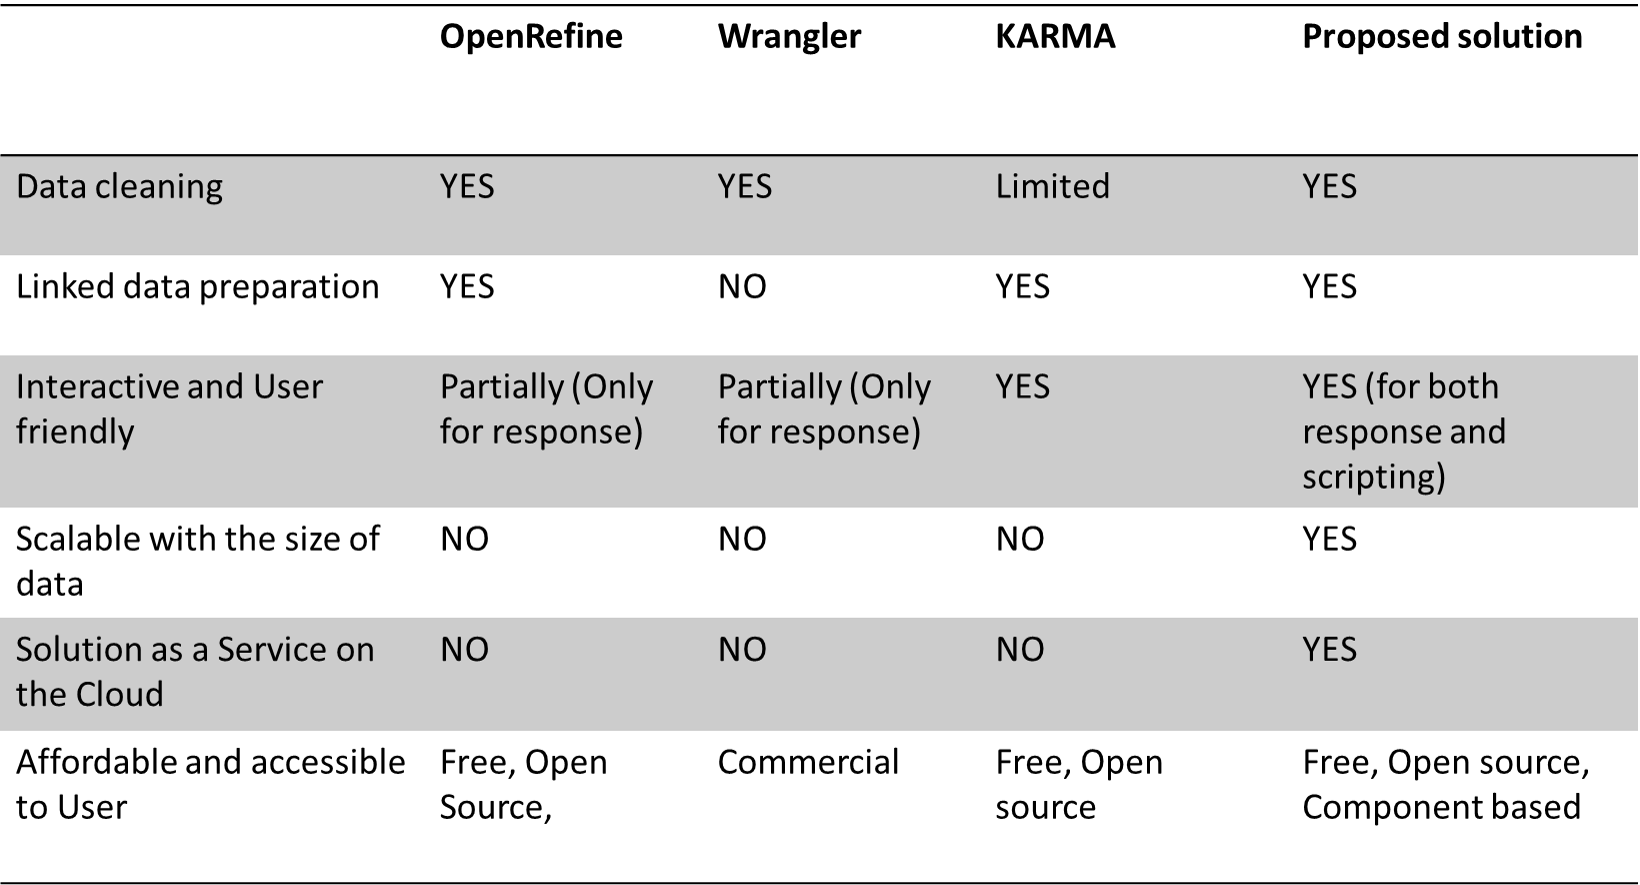
\includegraphics[width=38em]{./Figures/comparative_analysis}
	\begin{table}[htbp]
    \caption{Comparative analysis of relevant systems}
    \label{tab:2}
	\end{table}
\end{center}
\section{Escalated Requirements in Interactive Data Preparation}
\label{sec:requirements}
In this section, we discuss the important requirements which should be met by an integrated, interactive open data preparation solution apart from the main problem motivations. 
\subsection{Reusable and Repeatable cleaning}
\noindent A data transformation process can be performed on more than one data-set. Hence, it is important to have share-able data transformations between different data-sets, to save efforts spent on redundant data preparation process. Moreover, when a data cleaning is crowd-sourced, the need for capturing data alterations is increased \cite{2011-wrangler}.  Hence, the solution must keep track of how a data had been processed during the data cleaning process and should be share-able. 

\subsection{Sampling approaches of large volumes of data}
\noindent Processing large volumes of data takes significant amount of time, especially when it comes to iterative processes. This makes the interactivity between user actions and user feedback with user harder and more expensive to perform. For example, consider a scenario when a cleaning operation was performed wrongly and rolled-back. This leads to a significant waste of computing resources, especially if it was executed on large data. Big data processing requires rethinking traditional processes \cite{nemreport}. Correctness and efficiency are important attributes of data cleaning \cite{journals/corr/KrishnanW0FG16}. Sampling data-sets is a well-known technique of data cleaning and analysis \cite{Hellerstein08quantitativedata} for various purposes. This can be exploited in iterative cleaning of large data. Typically, sequential sampling (fetching an ordered subset) and random sampling (fetch subset from randomized data) are used to sample raw data. However, improper sampling can lead to wrong decisions \cite{journals/corr/KrishnanW0FG16}. For example a quantitative data may not able to spot outliers correctly if it is sampled sequentially (e.g. subset of first-N rows and calculate the average of sample), whereas random sampling produced more accurate results for aforementioned scenario \cite{Hellerstein08quantitativedata}. Sampling mechanism can depend on data being sampled, thus, allowing the user to choose the sampling technique according to input data provides accuracy and flexibility. Currently, data cleaning applications such as Wisteria \cite{Wisteria} and KARMA  \cite{knoblock15:aimag} use sampling for interactive data cleaning. However, user is unknown and not given an option to decide on sampling mechanism. The proposed solution should provide a feasible mechanism to sample input data, and allow user to decide on sampling approach. 
% \subsection{Separation between logical and physical implementations of data cleaning work-flow}
% \noindent Most data cleaning tools don't have clear separation of their logical and physical implementation of data transformation activities \cite{declarativedatacleaning}\cite{Wisteria}. Typically ETL work-flows are defined in high-level languages \cite{ETL}. This ceases from exploiting the logical query optimization which substantially results in inefficient and high-cost transformation work-flow for bigger data.  Logical query optimization is not possible unless otherwise the data worker consciously designs the cleaning work-flow accordingly \cite{ETL}. An automated mechanism to optimize cleaning work-flow can improve performance of data cleaning. 

\subsection{Flexibility}
\noindent Interactive data cleaning and transformations are often supported by underlying Domain Specific Languages (DSL) \cite{Wisteria}. They are typically less exposed and strongly typed. Although, the proposed system should support non-technical workers to do data cleaning, the optimal value can be achieved if the flexibility is given for customized transformation for technical users. 

